\documentclass[12pt,a4paper]{article}
\title{%
  Øving 6 \\
  \large IELET1001 - Elektroteknikk \\
  }
\author{Gunnar Myhre, BIELEKTRO}

\usepackage[utf8]{inputenc}
\usepackage[norsk]{babel}
\usepackage[siunitx]{circuitikz}
\usepackage{amsmath}
\usepackage{pgfplots}

\usepackage{graphicx}
\graphicspath{ {./images} }

\setlength\parindent{0pt}

\begin{document}
  \maketitle
    
  \section{Oppgåve 1}
    Straumen igjennom kondensatoren er gitt ved $i=C\frac{dv}{dt}$
    \begin{center}
      \begin{tabular}{ |c|c|c| }
        \hline
        $t$ & $\frac{dv}{dt}$ & $i$ \\
        \hline
        $[0,6\rangle$ & $12/6=2$ & $24A$ \\
        \hline
        $\langle6,10\rangle$ & $-20/4=-5$ & $-60A$ \\
        \hline
        $\langle10,16\rangle$ & $6/6=1$ & $48A$ \\
        \hline
      \end{tabular}
    \end{center}

    \begin{center}
      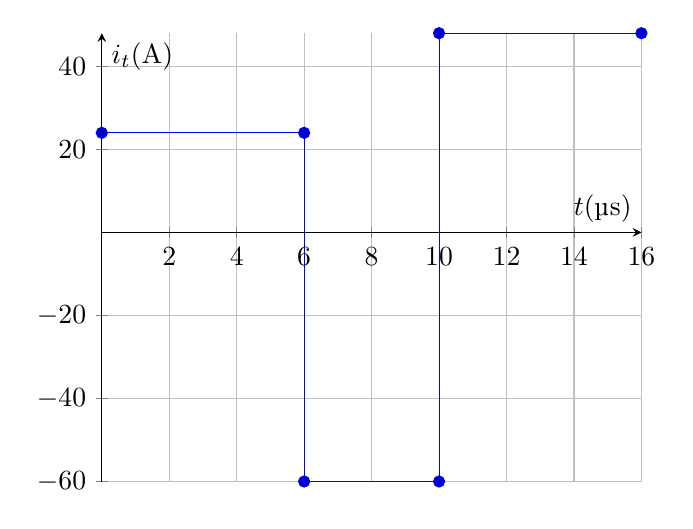
\begin{tikzpicture}
        \begin{axis}[axis lines=middle,grid=both,xlabel=$t(\si{\micro\s})$,ylabel=$i_{t}$(A)]
          \addplot coordinates{
            (0,24)    (6,24)
            (6,-60)   (10,-60)
            (10,48)   (16,48)
          };
        \end{axis}
      \end{tikzpicture}
    \end{center}

  \newpage

  \section{Oppgåve 2}
    Frå grafen kan vi lese verdiane av $i(t)$ for fire ulike intervaller
    \begin{center}
      \begin{tabular}{ |c|c| }
        \hline
        Intervall & $i(t)$ \\
        \hline
        $\langle 0, 2 \rangle$ & $7,5t$ \\
        \hline
        $\langle 2, 4 \rangle$ & $15$ \\
        \hline
        $\langle 4, 6 \rangle$ & $-15t$ \\
        \hline
        $\langle 6, 8 \rangle$ & $2,5t$ \\
        \hline
      \end{tabular}
    \end{center}
    Vi ser at formelen for energi lagra i kondensator kun er avhengig av
    kapasitansen \textbf{C} og spenninga \textbf{v}. Derfor kan vi svare på spørsmålet
    om $w_c(1,4)$ og $w_c(6,7)$ ved å finne $v_c(1,4)$ og $v_c(6,7)$.
    \begin{equation}
      w(t) = \frac{1}{2}Cv^2
    \end{equation}
    Formelen for spenning over kondensator er gitt ved
    \begin{equation}
      v(t) = v(t_0) + \frac{1}{C}\int_{t_0}^{t}i(t)dt
    \end{equation}
    \begin{itemize}
      \item $v_c(0) = 0$
      \item $v_c(2) = 0 + \frac{1}{5}\int_0^2 7,5tdt = 3V$
      \item $v_c(4) = 3 + \frac{1}{5}\int_2^4 15dt = 9V$
      \item $v_c(6) = 9 + \frac{1}{5}\int_4^6 -5dt = 7V$
    \end{itemize}
    Nå kan vi finne spenningene på dei to eksakte tidspunkta i oppgåveteksten, og
    deretter energien lagra ved desse tidspunkta.
    \begin{itemize}
      \item $v_c(1,4) = 0 + \frac{1}{5}\int_0^{1,4} 7,5tdt = 1,47V$
      \item $w_c(1,4) = \frac{5}{2}\si{\micro F}(1,47V)^2 = 5,402\si{\micro J}$
      \item $v_c(6,7) = 7 + \frac{1}{5}\int_4^{6,7} (2,5t - 5)dt = 6,423V$
      \item $w_c(6,7) = \frac{5}{2}\si{\micro F}(6,423)^2 = 103,121\si{\micro J}$
    \end{itemize}

    

  \section{Oppgåve 3}
    Spenningen over spolen er gitt ved $v=L\frac{di}{dt}$. Endringa i straumen over
    tid blir slik
    \begin{center}
      \begin{tabular}{ |c|c|c| }
        \hline
        $t$ & $\frac{di}{dt}$ & $i(t)$ \\
        \hline
        $[0,2\rangle$ & $4$ & $0A + 32/4A = 8A$ \\
        \hline
        $\langle2,4\rangle$ & $0$ & $8A+0A = 8A$ \\
        \hline
        $\langle4,6\rangle$ & $-4$ & $8A-32/4A = 0A$ \\
        \hline
        $\langle6,8\rangle$ & $0$ & $0A + 0A = 0A$ \\
        \hline
      \end{tabular}
    \end{center}

    \begin{center}
      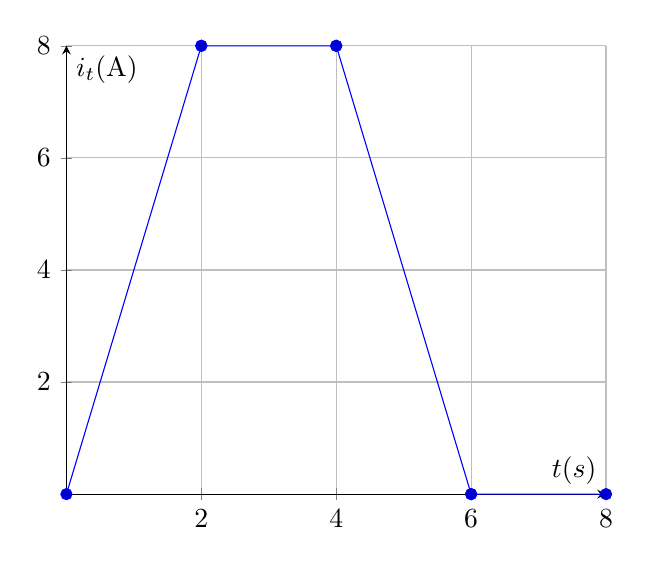
\begin{tikzpicture}
        \begin{axis}[axis lines=middle,grid=both,xlabel=$t(s)$,ylabel=$i_{t}$(A)]
          \addplot coordinates{
            (0,0)     (2,8)
            (2,8)     (4,8)
            (4,8)     (6,0)
            (6,0)     (8,0)
          };
        \end{axis}
      \end{tikzpicture}
    \end{center}

    \section{Oppgåve 4}
      \textbf{a)}
      \begin{equation}
        i(t) = 2sin(377t)A
      \end{equation}
      Deriverer uttrykket for $i(t)$
      \begin{equation}
        \frac{di}{dt} = 754cos(377t)A
      \end{equation}
      setter inn i formel for spenning over spole
      \begin{equation}
        v=L\frac{di}{dt} \rightarrow 100mH \cdot 754cos(377)A
      \end{equation}

      \textbf{b)}
      Bruker formel for energi i spole
      \begin{equation}
        w(t) = \frac{1}{2}Li^2(t)
      \end{equation}
      Setter inn for i og L
      \begin{equation}
        w(t) = \frac{1}{2}Li^2(t) \Rightarrow \frac{1}{20}(2sin(377t))
      \end{equation}

    \section{Oppgåve 5}
      \begin{center}
        \begin{circuitikz}[american] \draw
          (0,0) -- (3,0) -- (3,1)
                 to[C, l=14] (6,1) -- (6,0)
                 to[R, l=100<\ohm>] (9,0)
                 to[inductor, l=0.1<\henry>] (9,-3) -- (0,-3)
                 to[V, l=12V, invert] (0,0)
          (3,0) -- (3,-1)
                 to[R, l=250<\ohm>] (6,-1) -- (6,0)
          ;
        \end{circuitikz}
      \end{center}
      Ved stasjonære forhold vil spolen oppføre seg som ein kortslutning og
      kondensatoren som ein åpen krets. I dette tilfellet vil straumen igjennom
      kretsen vere gitt ved:
      \begin{equation}
        i=\frac{v}{R}=\frac{12V}{350\si{\ohm}} = 34,29mA
      \end{equation}
      Dette er også straumen igjennom spolen ved $t \rightarrow \infty$. Energien
      lagra i spolen er dermed gitt ved:
      \begin{equation}
        w(t)=\frac{1}{2}Li^2 \rightarrow \frac{1}{20}34,29^2\si{\henry\micro\ampere}
        = 58,79\si{\micro\joule}
      \end{equation}
      Spenninga over kondensatoren når $t\rightarrow \infty$ er gitt ved
      \begin{equation}
        v_c = \frac{250}{350}12V = 8,571V
      \end{equation}
      Sidan det er oppgitt at mengden energi lagra i kondensatoren er den same som
      i spolen kan vi nå finne kapasitansen til kondensatoren
      \begin{equation}
        w = \frac{1}{2}Cv^2 \rightarrow C = \frac{2\cdot 58,79}{8,751^2}
        = 1,60\si{\micro}F
      \end{equation}

    \newpage

    \section{Oppgåve 6}
      Ved stasjonære forhold vil spolene oppføre seg som kortslutningar og
      kondensatoren som ein åpen krets. Derfor kan vi forenkle kretsen slik:
      \begin{center}
        \begin{circuitikz}[american] \draw
          (0,0) to[V, l=15V, invert] (0,3) -- (3,3)
                to[R, l=3<\ohm>, *-] (6,3) -- (8,3)
                to[I, l=6A, invert] (8,0) -- (6,0)
                to[R, l=6<\ohm>] (6,3)
          (6,0) -- (0,0)
          ;
        \end{circuitikz}
      \end{center}
      som vi igjen kan forenkle v/kjeldetransformering:
      \begin{center}
        \begin{circuitikz}[american] \draw
          (0,0) -- (0,3)
                to[R, l=3<\ohm>] (2,3)
                to[R, l=6<\ohm>] (4,3)
                to[V, l=21V] (4,0) -- (0,0)
          ;
        \end{circuitikz}
      \end{center}

      \textbf{a)}
      Spenningsfallet over 3-ohm er $3/9 \cdot 21V = 7V$, effekten forbrukt i
      motstanden er gitt ved
      \begin{equation}
        P=\frac{v^2}{R} = \frac{7^2}{3} = 16,3W
      \end{equation}

      \textbf{b)}
      Ved $t\rightarrow \infty$ er spenninga over kondensatoren 15V. Energien lagra
      i kondensatoren er
      \begin{equation}
        w = \frac{1}{2}Cv^2 \rightarrow (15V)^2C = 225J
      \end{equation}

    \newpage

    \section{Oppgåve 7}
      \textbf{a)}
      Dei tri kondensatorane til høgre står i parallell (kondensator i parallell
      kan plussast saman).
      \begin{center}
        \begin{circuitikz}[american] \draw
          (0,0) -- (0,2)
                to[C, l=6<\micro F>] (0,4)
                to[C, l=6<\micro F>] (4,4) -- (4,2)
                to[C, l=18<\micro F>] (0,2)
          (4,2) -- (4,0)
                to[C, l=6<\micro F>] (0,0)

          (0,0) to[short, -o] (-1,0)
          (0,4) to[short, -o] (-1,4)
          ;
        \end{circuitikz}
      \end{center}
      $18 \si{\micro F}$ og den nederste $6 \si{\micro F}$ står i parallell $\rightarrow
      24 \si{\micro F}$. Denne står igjen i serie med den øverste $6\si{\micro F}$
      \begin{equation}
        \frac{6\cdot 24}{6+24}\si{\micro F} = 4,8 \si{\micro F}
      \end{equation}
      \begin{center}
        \begin{circuitikz}[american] \draw
          (0,0) to[C, l=6<\micro F>] (0,2) -- (2,2)
                to[C, l=4.8<\micro F>] (2,0) -- (0,0)

          (0,0) to[short, -o] (-1,0)
          (0,2) to[short, -o] (-1,2)
          ;
        \end{circuitikz}
      \end{center}
      \begin{equation}
        C_T = 10,8 \si{\micro F}
      \end{equation}

      \textbf{b)}
      Dei tri spolene til venstre er parallelle, og dei tri spolene til høgre
      er parallelle
      \begin{equation}
        \frac{12\cdot12}{12+12} = 6
      \end{equation}
      \begin{equation}
        \frac{6\cdot12}{6+12} = 4
      \end{equation}
      \begin{center}
        \begin{circuitikz}[american] \draw
          (0,0) to[inductor, l=12<\micro H>] (6,0) -- (6,2)
                to[inductor, l=4<\micro H>, -o] (4,2)
          (6,2) -- (6,4)
                to[inductor, l=12<\micro H>] (0,4) -- (0,2)
                to[inductor, l=4<\micro H>, -o] (2,2)
          (0,0) -- (0,2)
          ;
        \end{circuitikz}
      \end{center}
      Den øverste og den nederste spolen står i parallell $\rightarrow 6\si{\micro H}$.
      Nå står vi igjen med tri spoler i serie som vi kan legge saman:
      \begin{equation}
        L_T = 4 \si{\micro H} + 6 \si{\micro H}  + 4 \si{\micro H} = 14 \si{\micro H} 
      \end{equation}

    \section{Oppgåve 8.}
      Vi kan tolke ut ifrå informasjonen at kretsen var spenningssatt med $10V$ fram til
      $t=0s$ og deretter fråkopla med ein brytar. Det er derfor snakk om ein utladning
      frå $V(0) = V_s$ til $V(\infty)=0$, og dette kjenner vi formelen for:
      \begin{equation}
        v_c = V_{\infty} + \left(V_0 - V_{\infty} \right)e^{-\frac{t}{\tau}}
        = V_se^{-\frac{t}{\tau}}
      \end{equation}
      for $t > 0s$, $\tau = RC = 2s$ og $v_c = V$


      \textbf{a)} $v_c(1) = 10Ve^{-\frac{1}{2}} = 6,06V$


      \textbf{b)} $v_c(2) = 10Ve^{-\frac{2}{2}} = 3,68V$

    \section{Oppgåve 9}
      Ved $t=0$ lukker brytaren seg og kondensatoren begynner å lade seg opp.
      \begin{itemize}
        \item $v_c(0^-) = v_c(0^+) = 0V$
        \item Vi kan derfor sjå på $v_c$ som ein $0V$-spenningskjelde ved $t=0^+$,
          altså ein kortslutning. Då går ingen straum igjennom greina med $v_o$
          og $v_o(0^+) = 0V$
        \item Ved $t \rightarrow \infty$ vil kondensatoren oppføre seg som ein
          åpen krets. Då står vi igjen med tri motstandar i serie med $6V$-
          kjelda. Finner $v_o(\infty) = 3/10\cdot6V = 1,8V$ vha. spenningsdeling.
      \end{itemize}
      Vi finner $R_{th}$ frå kondensatoren ved å nulle ut spenningskjelda
      \begin{equation}
        R_{th} = \frac{2\cdot8}{2+8}\si{\kilo\ohm} = 1,8\si{\kilo\ohm}
      \end{equation}
      Dermed er $\tau = R_{th}C = 1,6\si{\kilo\ohm}\cdot 100\si{\micro F} = 160ms$.
      Nå kan vi sette inn i formel for RC-krets:
      \begin{equation}
        v_o(t)=v_o(\infty) + \left[ v_o(0^+)-v_o(\infty)\right] e^{-\frac{t}{\tau}}
        \rightarrow v_o(t) = 1,8 - 1,8e^{-t/0,16}V
      \end{equation}
      Som er uttrykket for spenninga over 3k-motstanden som vi var ute etter.

    \section{Oppgåve 10}
      Sidan vi antar at kretsen er stasjonær i $t=0$ vil spolen vere heilt opplada
      og oppføre seg som ein kortslutning. Finner $i_L(0^-)$ vha. maskestraum.
      \begin{itemize}
        \item $KVL_{I_s}: 10I_s - 6i_L = 6A$
        \item $KVL_{i_L}: 9i_L -  6I_s = 0$
      \end{itemize}
      Finner at ved $t=0^-$ er $I_s = 1A$ og $i_L = 2/3A$. Vi veit at straumen i ein
      spole ikkje kan endre seg brått
      \begin{equation}
        i_L(0^+) = 2/3A
      \end{equation}
      Ved $t \rightarrow \infty$ oppfører spolen seg som ein kortslutning. Uansett
      vil det ikkje gå nokon straumar i kretsen på dette tidspunktet sidan kjelda er
      avkopla. Derfor er $i_L(\infty) = 0A$. Vi finner $R_{th}$ for å finne
      tidskonstanten.
      \begin{itemize}
        \item $R_{th} = 9\si{\ohm}$
        \item $\tau = L/R_{th} = 2/9s = 0,22s$
      \end{itemize}
      Nå har vi alt vi trenger for å sette inn i formelen for RL-krets
      \begin{equation}
        i_l(t)=i_l(\infty) + \left[ i_l(0^+)-i_l(\infty)\right] e^{-\frac{t}{\tau}}
        \rightarrow i_l(t) = 0,667e^{-t/0,22}A
      \end{equation}
      Dette uttrykket $i_L(t)$ er kun gyldig for $t>0$. For $t<0$ har vi antatt at
      kretsen er stasjonær og $i_L = 0,667A$.
      \begin{center}
        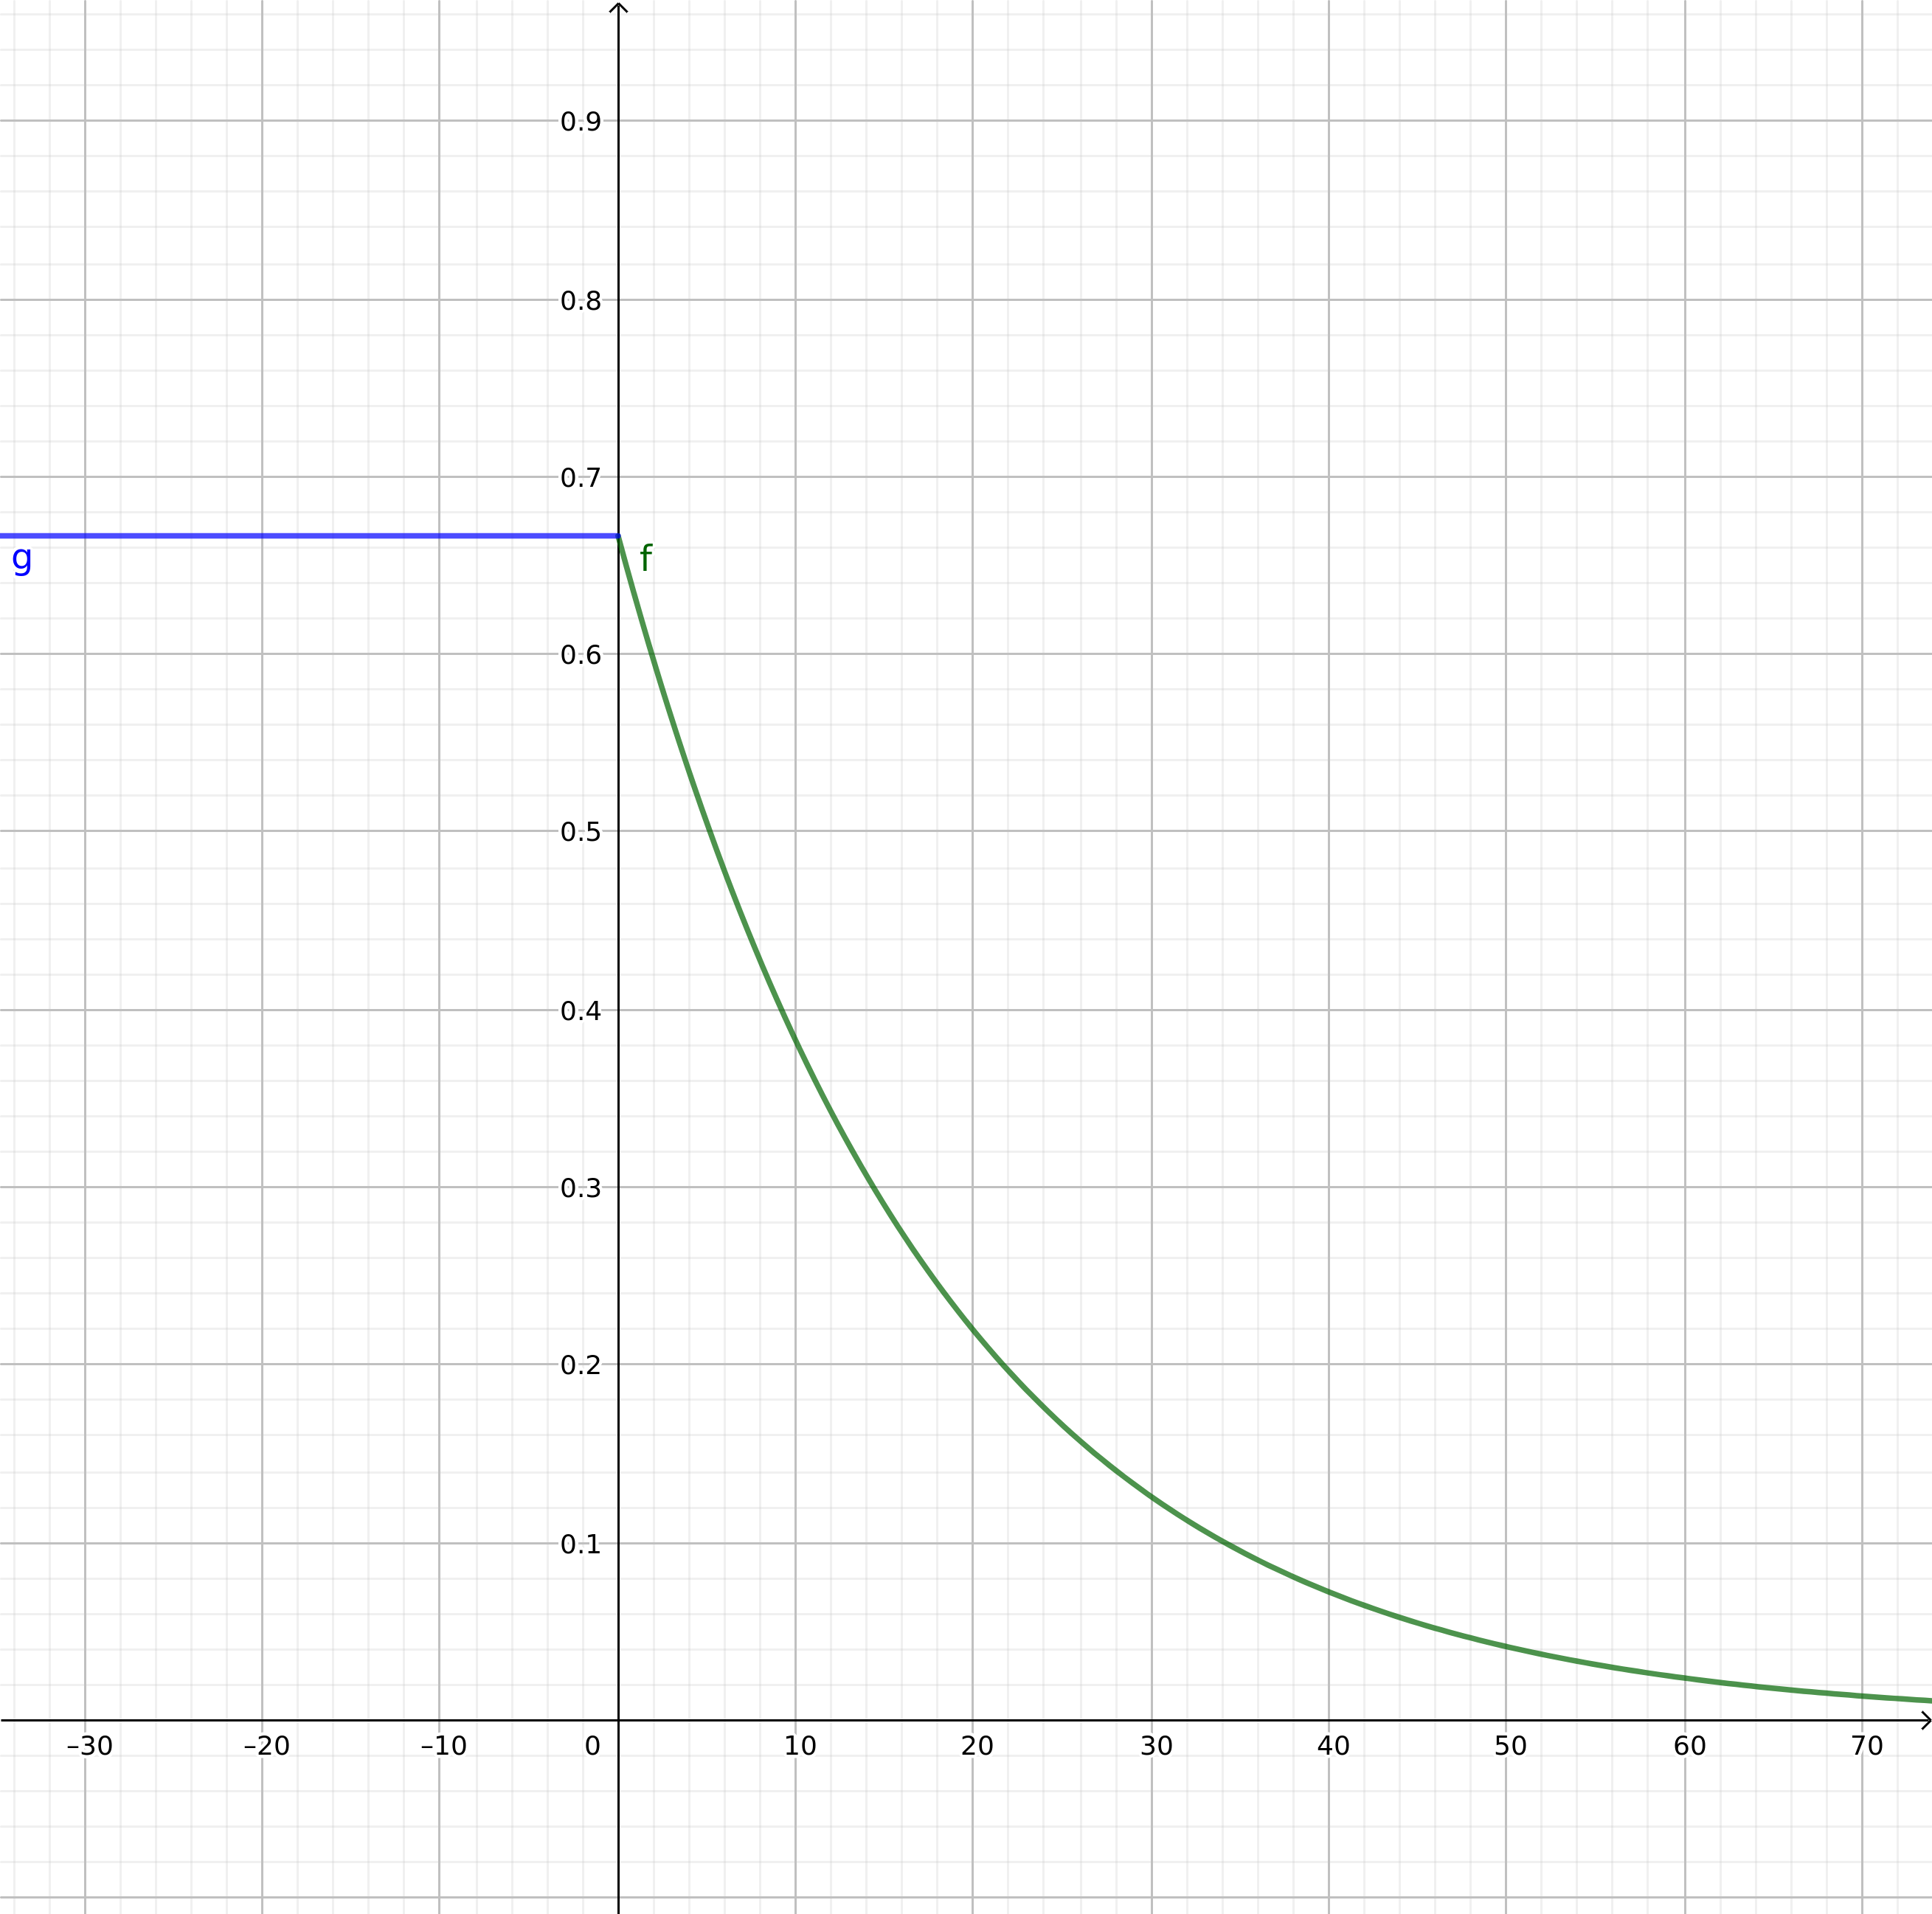
\includegraphics[width=200pt]{06_10.png}
      \end{center}

    \section{Oppgåve 11}
      Først kjeldetransformerer eg tri gonger for å fjerne to av motstandane på
      venstresida av kretsen som vi likevel ikkje er interesserte i verdiane til.
      \begin{center}
        \begin{circuitikz}[american] \draw
          (0,0) to[I, l=2<\ampere>] (0,3) -- (2,3)
                to[R, l=4<\ohm>] (2,0)
          (2,3) -- (4,3) 
                to[nos, invert] (4,0)
          (4,3) to[inductor, l=1H] (6,3)
                to[I, l=4<\ampere>, invert] (6,0)
          (6,3) -- (8,3)
                to[R, l=4<\ohm>, i=$i_o$] (8,0) --(0,0)
          ;
        \end{circuitikz}
      \end{center}
      \begin{itemize}
        \item \textbf{a)} Ved $t=0$ antar vi at kretsen er stasjonær, og spolen
          oppfører seg derfor som ein kortslutning. Vi kan dermed slå saman dei
          to straumkjeldene i parallell og finne $i_o$ ved straumdeling. Sidan
          motstandane har lik verdi vil halvparten av straumen gå i $i_o$, og vi
          får $i_o(0^+) = 3A$
        \item Ved $t\rightarrow \infty$ vil spolen også oppføre seg som ein
          kortslutning, då vil straumkjeldene stå i parallell med ein
          kortslutning (den lukka brytaren) og dermed vil all straumen gå der.
          Dette gjer at $i_o(\infty) = 0A$
        \item \textbf{b)} Tidskonstanten i ein RL-krets er gitt ved $\tau=L/R_{th}$.
          Vi finner $R_{th}$ ved å sjå på kretsen når $t>0$. Sidan brytaren er lukka
          og vi nuller ut kjeldene vil spolen kun stå i serie med éin av motstandane.
          Den andre er kortslutta av brytaren. $R_{th} = 4\si{\ohm}$ og
          $\tau = L/R_{th} = 0,25s$
      \end{itemize}
      \textbf{c)} Ved å sette inn i formel for RL-krets finner vi uttrykket
      \begin{equation}
        i_o(t)=i_o(\infty) + \left[ i_o(0^+)-i_o(\infty)\right] e^{-\frac{t}{\tau}}
        \rightarrow i_o(t) = 3e^{-t/0,25}A
      \end{equation}
      \begin{center}
        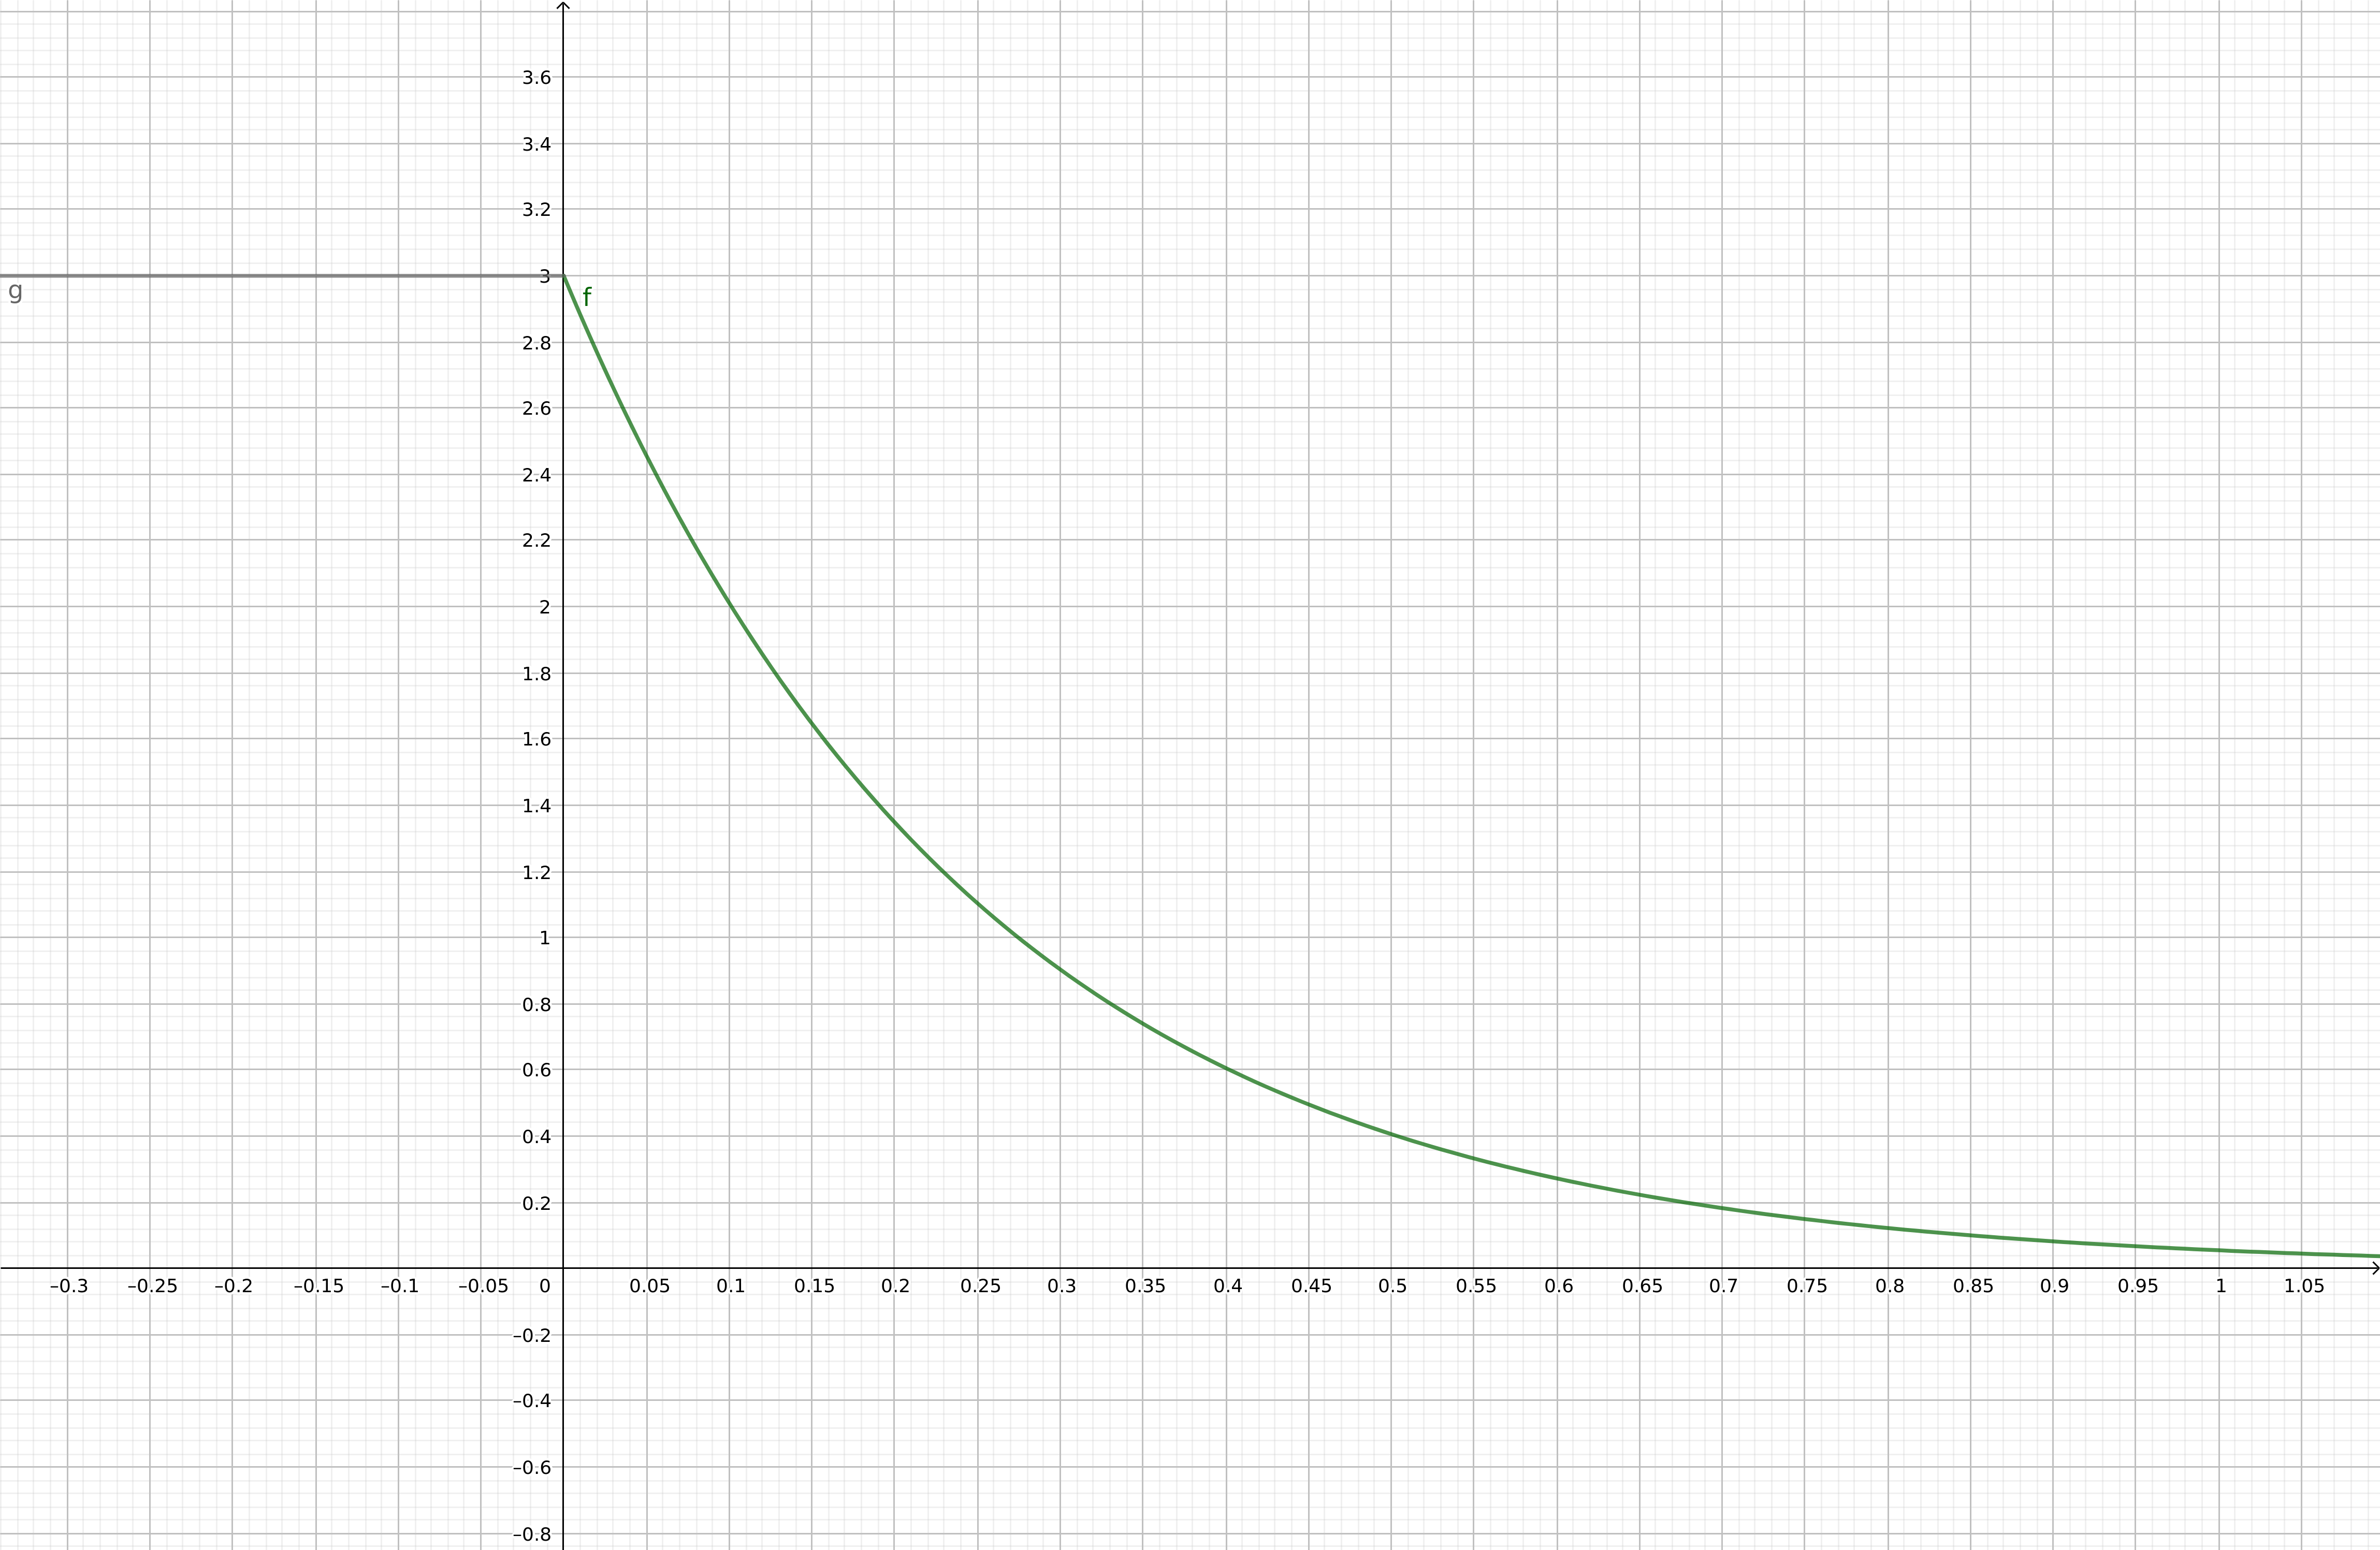
\includegraphics[width=200pt]{06_11.png}
      \end{center}
      (I denne oppgåva har eg kanskje gjort feil sidan $1H$ må sjåast på som ein
      straumkjelde for tilstanden $t = 0^+$.)

    \section{Oppgåve 12}
      \textbf{a)}
      Ved $t=0^-$ antar vi at kretsen er stasjonær og kondensatoren oppfører seg som
      ein åpen krets. Bruker nodespenning i kretsen ved $t = 0^-$ for å finne spenninga
      over kondensatoren, $v_c(0^-)$, og straumen $i_o(0^-)$
      \begin{center}
        \begin{circuitikz}[american] \draw
          (0,0) to[R, l=3<\kilo\ohm>] (0,6) -- (2,6)
                to[R, l=1<\kilo\ohm>] (2,3)
                to[V, l=$6V$] (2,0)
          (2,6) -- (4,6)
                to[R, l=1<\kilo\ohm>] (4,3)
                to[R, l=1<\kilo\ohm>, i=$i_o(0^-)$] (4,0) -- (0,0)

          (2,3) to[open, v=$v_c(0^-)$] (4,3)
          (2,6) node[label={[font=\footnotesize]100:$1$}] {}
          (4,3) node[label={[font=\footnotesize]100:$2$}] {}
          ;
        \end{circuitikz}
      \end{center}
      \begin{itemize}
        \item $KCL_1: 15v_1 - 3v_2 = 72$
        \item $KCL_2: -v_1 + 3v_2 = 0$
        \item $v_c(0^-) = 6V - v_2$
      \end{itemize}
      Løyser likningssettet og får at $v_c(0^-) = 4,67V$. Sidan spenninga over
      ein kondensator er kontinuerleg kan vi sette $v_c(0^+) = 4,67V$ som ein
      spenningskjelde for kretsen i tidspunktet $t=0^+$. Løyser denne kretsen
      vha.  maskestraum. (Kretsen her er lik teikninga i oppgåveteksten, men
      med brytaren lukka og kondensatoren bytta ut med ein spenningskjelde med
      polaritet som vist i teikninga over.)
      \begin{itemize}
        \item $KVL_a: 4I_a -I_b + 6 = 0$
        \item $KVL_b: 5I_b - I_a - I_d - 4,67 = 0$
        \item $KVL_c: 2I_c - 2I_d - 6 + 4.67 = 0$
        \item $KVL_d: 6I_d - 2I_c - 4I_b = 0$
        \item $i_o(0^+) = i_c - i_d$
      \end{itemize}
      Løyser likningssettet og finner $i_o(0^+) = 0,66A$. Ved $t \rightarrow \infty$
      er kretsen stasjonær igjen og kondensatoren oppfører seg som ein åpen krets.
      Greina med $i_o$ er kortslutta av greina med brytaren, derfor er $i_o(\infty) = 0$. \\

      \textbf{b)}
      For ein RC-krets er $\tau = RC = R_{th}C$. $R_{th}$ frå kondensatoren for $t>0$ er 
      $1,33\si{\kilo\ohm}$, så tidskonstanten $\tau = 1,33\si{\kilo\ohm} \cdot 150
      \si{\micro F} = 200ms$. \\
      
      \textbf{c)}
      Vi kan finne eit uttrykk for $i_o(t)$ som er avhengig av $v_c(t)$
      \begin{equation}
        i_o(t) = \frac{v}{R} = \frac{6V - v_c(t)}{2\si{\kilo\ohm}}
      \end{equation}
      dette kan vi utfylle med uttrykk for $v_c(t)$. Vi veit at $v_c(0^+) = 4,67V$, og
      sidan greinene med 4k- og 2k-motstandane er kortslutta av brytaren for $t>0$ er
      spenninga over kondensatoren $6V$ for $t \rightarrow \infty$
      \begin{equation}
        v_c(t) = v_c(\infty) + \left[ v_c(0^+) - v_c(\infty) \right] e^{-t/\tau}
        \Rightarrow 6V - 1,33e^{-t/\tau}
      \end{equation}
      setter inn for $v_c(t)$
      \begin{equation}
        i_o(t) = \frac{6V - v_c(t)}{2\si{\kilo\ohm}} \rightarrow
        \frac{6V - (6V - 1,33e^{-t/\tau})}{2\si{\kilo\ohm}} \rightarrow
        \frac{1,33e^{-t/200\cdot 10^{-3}}}{2\si{\kilo\ohm}}
      \end{equation}

      \textbf{d)}
      \begin{center}
        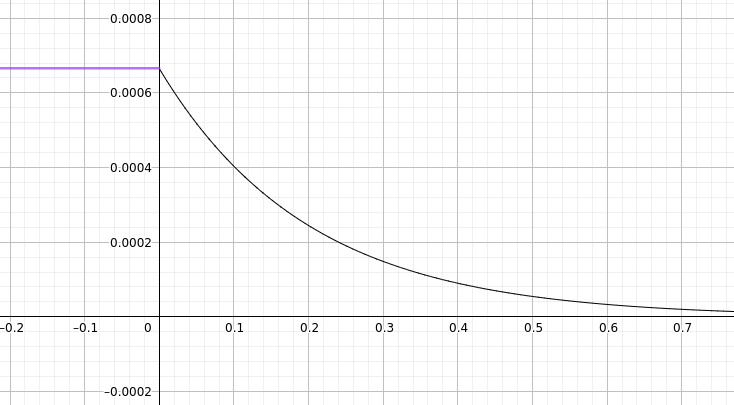
\includegraphics[width=300pt]{06_12.png}
      \end{center}

\end{document}
